\documentclass{beamer}
\usepackage{ragged2e}
\usepackage{listings}
\usepackage{textcomp}
\usepackage{multicol}
\justifying

\usetheme{CambridgeUS}
\usecolortheme{beaver}

\title[SM SysId with EE noise structure]{
    \Large\textbf{LABORATORY OF ROBUST IDENTIFICATION AND CONTROL}
}
%{\textbf{Lab \#2: Set-Membership System Identification with Equation Error noise structure \\
%(Unknown But Bounded noise)}}

\subtitle{Lab\#2 Solution}

\author[Carlo Migliaccio]{Carlo Migliaccio}

\institute[PoliTO]{Master's Degreee in Computer Engineering\\
Politecnico di Torino}

\date{October 2024}

\AtBeginSection[]{
    \begin{frame}
        \frametitle{Set-Membership Identification with EE noise structure}
    \tableofcontents[currentsection]
    \end{frame}
}


\begin{document}
\maketitle
\begin{frame}
    \frametitle{Set-Membership Identification with EE noise structure}
    \tableofcontents
\end{frame}

\section{Problem 1: FPS mathematical formulation}
\begin{frame}
    \frametitle{Problem 1: description}
    In this problem we assume that the plant to be identified is exactly described as a discrete-time LTI model as follows:
    \begin{equation}\label{eq:model}
        G_p(q^{-1})=\frac{\theta_2}{1+\theta_1{q^{-1}}}
    \end{equation}
    where $\theta=[\theta_1 \ \theta_2]=[-0.5 \ 2]$
    Assume that the uncertainty affecting the input-output data enters the problem according to an \textbf{Equation-Error (EE)} structure. Furthermore, to perform the simulation assume that:
    \begin{equation}
        \tilde{u}=[4,-3,2,1]^T \quad 
        e=[0.05,-0.25, 0.3, -0.5]
    \end{equation}
    Perform a simulation of model (\ref{eq:model}) in order to simulate the experiment. The equation to be used is the following: 
    \begin{equation}
        \tilde{y}(k)=-\theta_1\tilde{y}(k-1)+\theta_2\tilde{u}(k)+e(k), \quad \tilde{y}(1)=0
    \end{equation}
    where $e$ is such that $\vert e(k) \vert \le \Delta_e$, $\Delta_e=0.5$\\
\end{frame}

\begin{frame}
    \frametitle{Problem 1: FPS mathematical formulation (task 1)}
    \begin{alertblock}{Task 1}
        \justifying
        {Assuming that the bound $\Delta_e$ is the only available information on the error e, provide the implicit mathematical definition of the feasible parameter set (FPS) $\mathcal{D}_\theta$ for the considered Set-Membership System Identification problem.}
    \end{alertblock}
    \begin{equation}
        \begin{aligned}
            \mathcal{D}_\theta=\{
                &\theta\in\mathbb{R}^2: \tilde{y}(k)+\theta_1\tilde{y}(k-1)-\theta_2{\tilde{u}(k)}=e(k), k=2,3,4\\
                &\vert e(k) \vert \le \Delta_e \ k=1,...,4 
            \}=\\
            &\{
                \theta \in \mathbb{R}^2: \vert \tilde{y}(k)+\theta_1\tilde{y}(k-1)-\theta_2{\tilde{u}(k)} \vert \le \Delta_e, \ k=2,3,4
            \}=\\
            &\{
                \theta \in \mathbb{R}^2: -\Delta_e \le \tilde{y}(k)+\theta_1\tilde{y}(k-1)-\theta_2{\tilde{u}(k)} \le \Delta_e, \\ &k=2,3,4
            \}=\{
                \theta\in\mathbb{R}^2: 
                {\color{red}\theta_1\tilde{y}(k-1)-\theta_2{\tilde{u}(k)} \le \Delta_e -\tilde{y}(k)},\\
                &{\color{blue}-\theta_1\tilde{y}(k-1)+\theta_2{\tilde{u}(k)} \le \Delta_e +\tilde{y}(k)}
            \} \Longrightarrow \text{\small(see next slide)}
        \end{aligned}
    \end{equation}
\end{frame}

\begin{frame}
    \frametitle{Problem 1: FPS mathematical formulation (task 1)}
    \begin{equation*}
        \mathcal{D}_\theta=\{
            \theta\in\mathbb{R}^2: A\theta\le{b} 
        \}\quad \text{bounded polyhedron} \to \text{\color{red} \textbf{POLYTOPE}}
    \end{equation*}
    where $A$, $\theta$, $b$ are such that:
    \begin{equation}\label{eq:ineq}
        \underbrace{\begin{bmatrix}
            \tilde{y}(k-1)&-\tilde{u}(k)\\
            -\tilde{y}(k-1)&\tilde{u}(k)
        \end{bmatrix}}_{A} \underbrace{\begin{bmatrix}
            \theta_1\\
            \theta_2
        \end{bmatrix}}_\theta \le \underbrace{\begin{bmatrix}
            \Delta_e-\tilde{y}(k)\\
            \Delta_e+\tilde{y}(k)
        \end{bmatrix}}_{b} \quad k=2,3,4
    \end{equation}
    In particular: 
    \begin{equation}\label{eq:data}
        A=\begin{bmatrix}
            0&3\\
            -6.25&-2\\
            1.175&-1\\
            0&-3\\
            6.25&2\\
            -1.175&1
        \end{bmatrix}, \quad
        b=\begin{bmatrix}
            6.75\\
            -0.675\\
            -1.5875\\
            -5.75\\
             1.675\\
             2.5875
        \end{bmatrix}
    \end{equation}
\end{frame}

\begin{frame}
    \frametitle{Problem 1: Graphical representation of the FPS (task 2)}
    \begin{alertblock}{Task 2}
        \justifying
        Provide a graphical representation of obtained FPS and analyze its geometrical features.
    \end{alertblock}
    By using the (\ref{eq:ineq}) and substituting the data in  (\ref{eq:data}) we obtain the following set of  inequalities: 
    \begin{equation}
        \begin{cases}
            &3\theta_2\le6.75\\
            &-6.25\theta_1-2\theta_2\le-0.675\\
            &1.175\theta_1-\theta_2\le-1.5875\\
            &-3\theta_2\le-5.75\\
            &6.25\theta_1+2\theta_2\le1.675\\
            &-1.175\theta_1+\theta_2\le2.5875
        \end{cases}
    \end{equation}
\end{frame}

\begin{frame}
    \frametitle{Problem 1: Graphical representation of the FPS (task 2)}
    In the $\mathbb{R}^2$ plane, each one of the inequalities is an halfplane. If we take their intersection we obtain an $\mathbb{R}^2$-polytope which represents the FPS $\mathcal{D}_\theta$, the one indicated in {\color{orange} orange}.

    \begin{multicols}{2}
        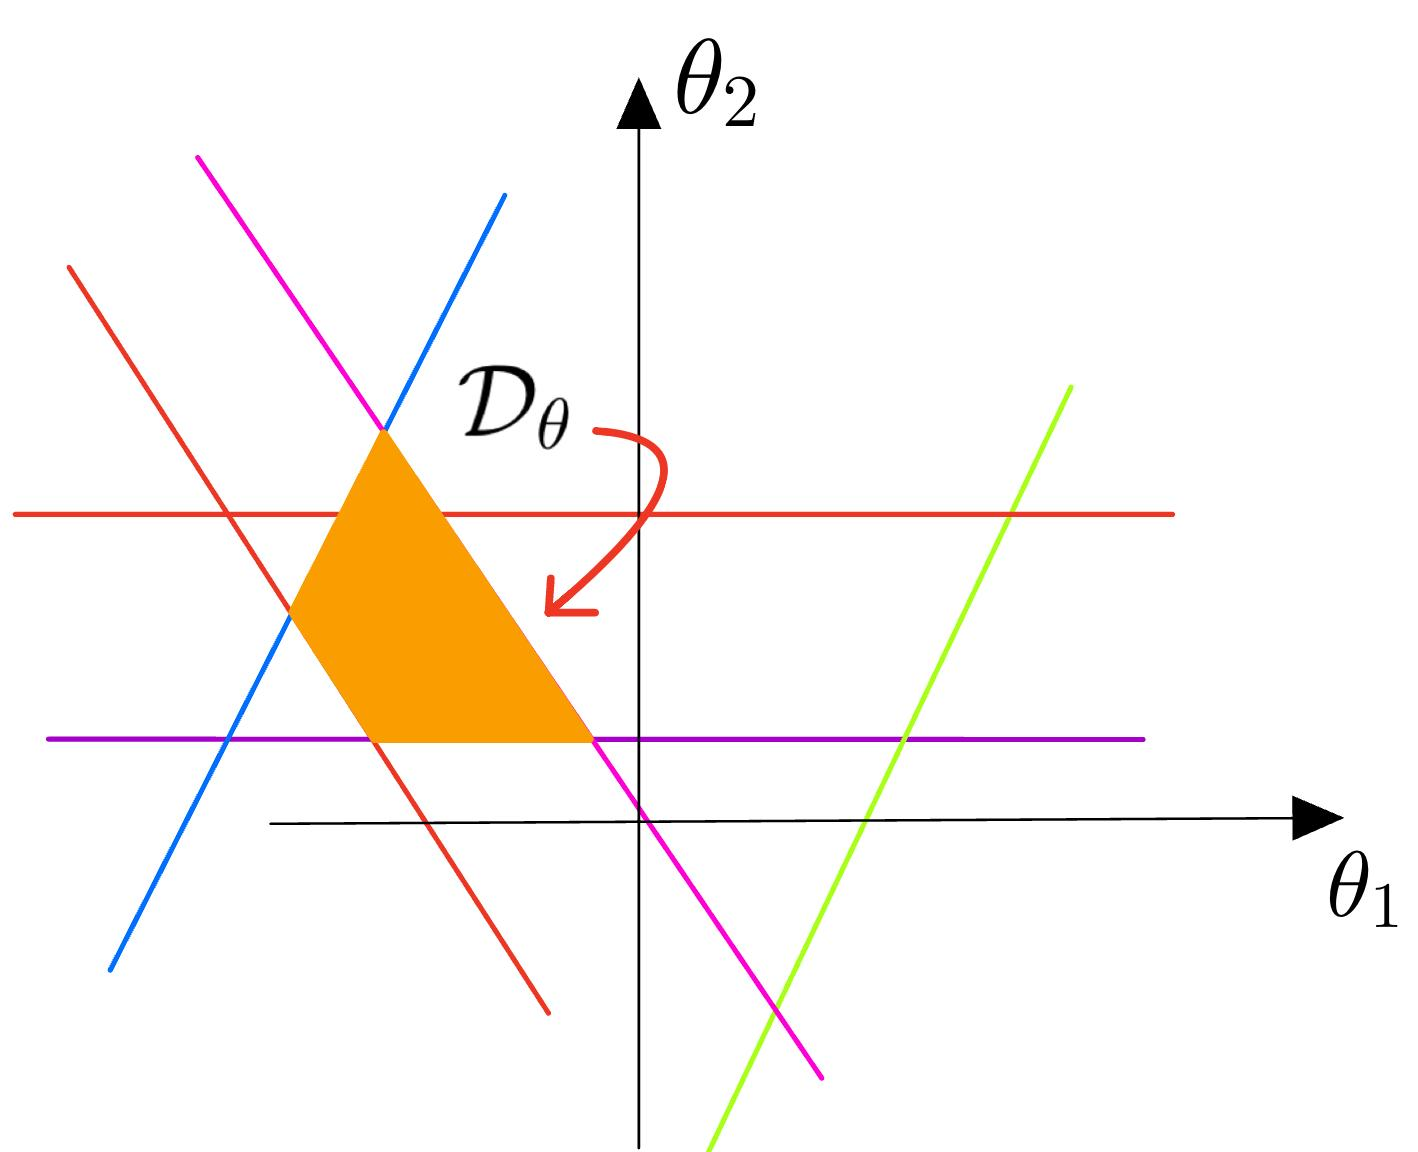
\includegraphics[scale=0.12]{img/polytope.jpeg}\\
        \newcolumn
        At this point the following \textbf{optimization problems} have to be solved. \\\alert{For the $PUI_{\theta_1}$}
        \vspace{-0.3cm}
        \begin{align}
            &\underline{\theta}_1  = \min_{\theta\in\mathcal{D}_\theta} \theta_1 \\
            &\overline{\theta}_1 = -\min_{\theta\in\mathcal{D}_\theta} -\theta_1 
        \end{align}
        \vspace{-0.3cm}
        \alert{For the $PUI_{\theta_2}$}
        \begin{align}
            &\underline{\theta}_2  = \min_{\theta\in\mathcal{D}_\theta} \theta_2 \\
            &\overline{\theta}_2 = -\min_{\theta\in\mathcal{D}_\theta} -\theta_2
        \end{align}
    \end{multicols}
\end{frame}

\begin{frame}
    \frametitle{Problem 1: PUI computation (task 3 )}
    \begin{alertblock}{Task 3}
        \justifying
        Exploiting the obtained geometrical description, compute the parameter uncertainty interval $PUI_{\theta_1}$ and $PUI_{\theta_2}$
    \end{alertblock}
    By using \textsc{MATLAB}, and outerbounding the polytope with a {\color{red}rectangle}, we can say that approximately the $PUI$s are those shown in the following figure:
    \begin{multicols}{2}
        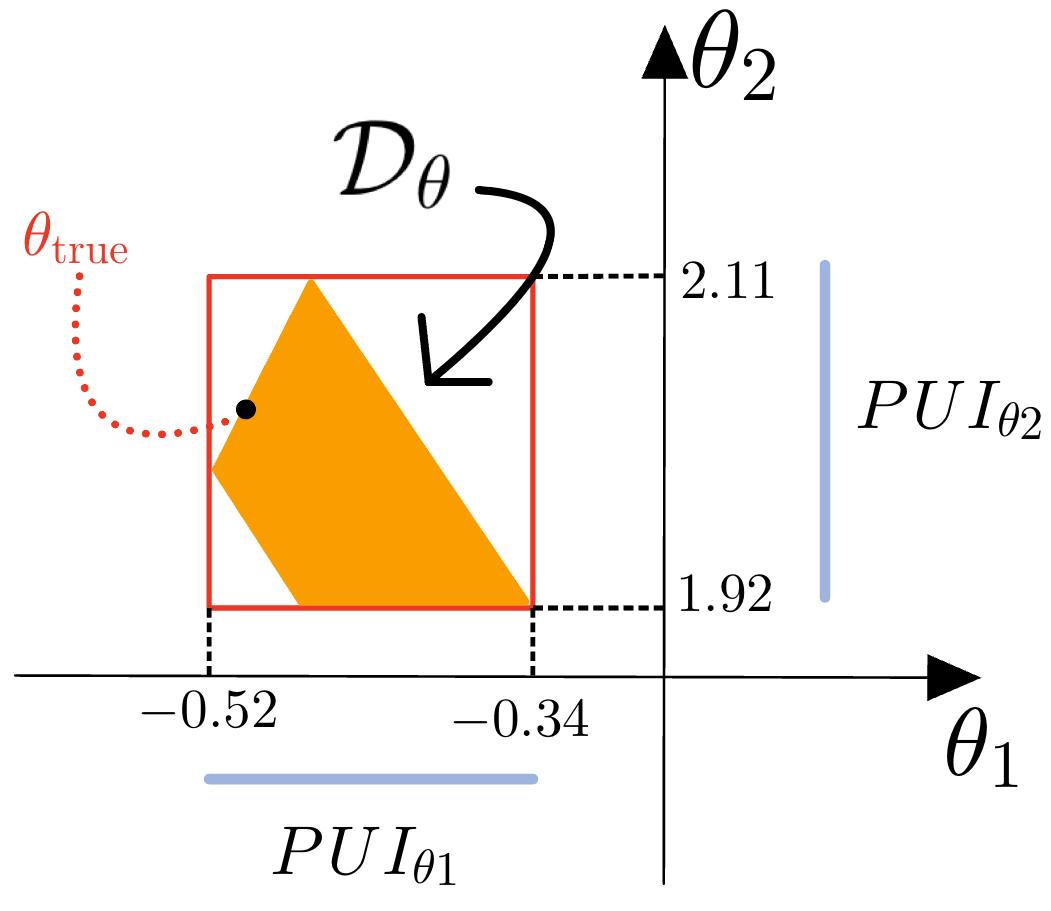
\includegraphics[scale=0.13]{img/pui.jpeg}\\
        \newcolumn
        The $PUI$s are then approximately: 
        \begin{align}
            &PUI_{\theta_1}=[-0.52,-0.34]\\
            &PUI_{\theta_2}=[1.92, 2.11]
        \end{align}
        Note that \alert{$\theta_{\text{true}}=[-0.5,2]$} is on the border of the computed $\mathcal{D}_\theta$. This is important for the SM Identification approach.
    \end{multicols}
\end{frame}


\section{Problem 2: PUI computation and Linear Programming}
\begin{frame}
    \frametitle{Problem 2: description}
    In this problem we assume that the plant to be identified is exactly described as a DT LTI model whose transfer function is: 
    \begin{equation}\label{eq:sys2}
        G_p(q^{-1}) = \frac{N(q^{-1})}{D(q^{-1})}=
        \frac{\theta_3+\theta_4{q^{-1}}+\theta_5{q^{-2}}}{1+\theta_1{q^{-1}}+\theta_2{q^{-2}}} 
    \end{equation}
    where $\theta=[\theta_1\ \theta_2 \ \theta_3 \ \theta_4  \theta_5 ] = [-0.7647, 0.3012, 0, 32.24, 21.41]$. 
    The objective here is to compute a Set-Membership estimation of the model parameters. The data are collected by simulating the system (\ref{eq:sys2}). In particular, as far as the input is concerned, it is a random sequence uniformly distributed in $[0,1]$, while the error is a random sequence uniformly distributed in $[-\Delta_e, \Delta_e]$\footnote{
        Different $\Delta_e$ must be used from 0.1 to 100
    }.
    The output sequence must be computed as follows: 
    \begin{equation}
        y(k)=-\theta_1{y(k-1)}-\theta_2{y(k-2)}+\theta_3{u(k)}+\theta_4{u(k-1)}+\theta_5{u(k-2)} + e(k)
    \end{equation}
\end{frame}

\begin{frame}
    \frametitle{Problem 2: Feasible Parameter Set $\mathcal{D}_\theta$ definition}
    \framesubtitle{Main ingredients}
    \begin{itemize}
        \item \textit{A-priori information on the system}: \textbf{second order} (n=2), \textbf{linear time-invariant (LTI)}; 
        \item \textit{A-priori information on the noise}: 
        \begin{enumerate}
            \item Noise structure: the uncertainty enters into the identification problem as an additive term (equation-error), then the same as before; 
            \item Noise property: the noise samples are bounded, that is $\vert e(k) \vert \le \Delta_e$, $k=1,...,N$, the bound $\Delta_e$ is known
        \end{enumerate}
        \item \textit{A-posteriori information}: data generated by simulating the system with randomly generated $u(k)$ and $e(k)$.
    \end{itemize}
\end{frame}

\begin{frame}
    \frametitle{Problem 2: Feasible Parameter Set $\mathcal{D}_\theta$ definition}
    \framesubtitle{Implicit mathematical formulation}
    
    \begin{alertblock}{Task 1}
        \justifying
        Define the feasible parameter set (FPS) $\mathcal{D}_\theta$ for the considered set-membership identification problem.
    \end{alertblock}
    \begin{equation}
        \begin{aligned}
            \mathcal{D}_\theta=
        \{
            &\theta\in\mathbb{R}^5: \ 
            y(k)=-\theta_1{y(k-1)}-\theta_2{y(k-2)}+\\
            &+\theta_3{u(k)}+\theta_4{u(k-1)}+\theta_5{u(k-2)} + e(k), \ k=3,...,N\\
            &\vert e(k) \vert \le \Delta_e, \ k=1,...,N
        \}=\\
        \{
            &\theta\in\mathbb{R}^5: \ 
            y(k)+\theta_1{y(k-1)}+\theta_2{y(k-2)}+\\
            &-\theta_3{u(k)}-\theta_4{u(k-1)}-\theta_5{u(k-2)}= e(k), \ k=3,...,N\\
            &\vert e(k) \vert \le \Delta_e, \ k=1,...,N
        \} \Longrightarrow \text{\small{(see next slide)}}
        \end{aligned}
    \end{equation}
\end{frame}

\begin{frame}
    \frametitle{Problem 2: Feasible Parameter Set $\mathcal{D}_\theta$ definition}
    \framesubtitle{Implicit mathematical formulation}
    By eliminating the dependence on $e(k)$ samples, the set is rewritten as: 
    \begin{equation}\label{eq:FPS}
        \begin{aligned}
           \mathcal{D}_\theta= \{
            &\theta\in\mathbb{R}^5: \ 
            \vert y(k)+\theta_1{y(k-1)}+\theta_2{y(k-2)}+\\
            &-\theta_3{u(k)}-\theta_4{u(k-1)}-\theta_5{u(k-2)}\vert \le \Delta_e, \ k=3,...,N
        \}=\\
        \{
            &\theta\in\mathbb{R}^5: \
            {\color{red}\theta_1{y(k-1)}+\theta_2{y(k-2)}+}\\
            &{\color{red}-\theta_3{u(k)}-\theta_4{u(k-1)}-\theta_5{u(k-2)} \le \Delta_e - y(k)}\\
            &{\color{orange}-\theta_1{y(k-1)}-\theta_2{y(k-2)}+}\\
            &{\color{orange}+\theta_3{u(k)}+\theta_4{u(k-1)}+\theta_5{u(k-2)} \le \Delta_e + y(k)}, \ k=3,...,N
        \}
        \end{aligned}
    \end{equation}
    This describes implicitly \alert{all the possible solutions} for our identification problem, since for each choice of $\theta$ coherent with $\mathcal{D}_\theta$, I obtain a different model.
\end{frame} 

\begin{frame}
    \frametitle{Problem 2: Feasible Parameter Set $\mathcal{D}_\theta$ definition}
    \framesubtitle{Computing the Parameter Uncertainty Intervals (PUIs)}
    Provided that the Feasible Parameter Set has been formulated as in (\ref{eq:FPS}), the problem of computing the PUI can be written as follows: 
    \begin{definition}[\textbf{Parameter Uncertainty Interval (PUI)}]
        For each parameter $\theta_j$ the $PUI_{\theta_j}$ is defined as follows:
        \begin{equation}
            PUI_{\theta_j} =[\underline{\theta}_j, \overline{\theta}_j]
        \end{equation}
        where: 
        \begin{align}\label{eq:opt_prob}
            \underline{\theta}_j = \min_{\theta\in\mathcal{D}_\theta} \theta_j, \quad 
            \overline{\theta}_j = \max_{\theta\in\mathcal{D}
            _\theta} \theta_j \Rightarrow 
            \overline{\theta}_j = -\min_{\theta\in\mathcal{D}_\theta} -\theta_j
        \end{align}
    \end{definition}
    
\end{frame}

\begin{frame}
    \frametitle{Problem 2: Feasible Parameter Set $\mathcal{D}_\theta$ definition}
    \framesubtitle{PUI computation by means of Linear Programs (LP) solution}
    %---------------------------------------
    The set in (\ref{eq:FPS}) can be rewritten in a more-compact matrix form as: 
    \begin{equation}
        \mathcal{D}_\theta = \{
            \theta \in \mathbb{R}^5: A\theta\le{b}
        \}
    \end{equation}
    where: 
    {\small{
        \begin{align*}
            &A=\begin{bmatrix}
                {y(k-1)}&{y(k-2)}&-{u(k)}&-{u(k-1)}&-{u(k-2)}\\
                -{y(k-1)}&-{y(k-2)}&{u(k)}&{u(k-1)}&{u(k-2)}\\
            \end{bmatrix}, \\
            &b=\begin{bmatrix}
                \Delta_e - y(k)\\
                \Delta_e + y(k)
            \end{bmatrix}, \quad 
            k=3,...,N
        \end{align*}
    }}We have seen that the derived set is a polytope that is a convex one, moreover the objective of the problems in (\ref{eq:opt_prob}) is also convex (in particular is linear). The \alert{minimization of a \textbf{linear objective} over a \textbf{polytope}} raises a problem of \alert{\textbf{Linear Programming (LP)}}. Well known algorithms (eg. \textit{Barrier method}) have been developed in order to solve such problems.
\end{frame}


\begin{frame}[fragile]
    \frametitle{Problem 2: Feasible Parameter Set $\mathcal{D}_\theta$ definition}
    \framesubtitle{PUI computation by means of Linear Programs (LP) solution}
    The problems in (\ref{eq:opt_prob}) can be rewritten as:
    \begin{align}
            &\underline{\theta}_j = \min_{\theta}{c^T{\theta}} \ &\text{subject to:} \ A\theta\le{b} \\
            &\overline{\theta}_j = \max_{\theta}{c^T{\theta}} \ &\text{subject to:} \ A\theta\le{b}
    \end{align}
    where $c_i=1 \iff i=j$. Linear Programming solvers can be used in order to find a \alert{global optimal solution.} In MATLAB the \texttt{linprog()} command can be used.
    \begin{exampleblock}{MATLAB$^\text{\tiny\textregistered}$ Code}\justifying
        \small
         In the following there is an example of MATLAB code for the computation of $PUI_{\theta_1}$
        {\tiny{
            \begin{verbatim}
    A=[y(2:N-1) y(1:N-2) -u(3:N) -u(2:N-1) -u(1:N-2); 
    -y(2:N-1) -y(1:N-2) u(3:N) u(2:N-1) u(1:N-2)];
    b=[dE*ones(N-3+1)-y(3:N); dE*ones(N-3+1)+y(3:N)];
    c=zeros(5,1); c(1)=1; 
    [~,th1_inf] = linprog(c,A,b); 
    [~,th1_sup] = linprog(-c,A,b); th1_sup=-th1_sup;
                        \end{verbatim}
        }}
    \end{exampleblock}
\end{frame}

\begin{frame}
    \frametitle{Problem 2: Feasible Parameter Set $\mathcal{D}_\theta$ definition}
    \framesubtitle{PUI computation by means of Linear Programs (LP) solution}

    Choosing $\Delta_e=10$ the following PUIs have been computed:
    \begin{table}
        \centering
        \begin{tabular}{c c c c c}
             &$\underline{\theta}_j$&$\overline{\theta}_j$&$\theta_j^c$&$  \theta_{\text{true}}$\\
            \hline\hline
            $PUI_{\theta_1}$\vline\vline&-0.7984&-0.7303&-0.76438&-0.7647\\
            $PUI_{\theta_2}$\vline\vline&0.2690&0.3354&0.3022&0.3012\\
            $PUI_{\theta_3}$\vline\vline&-1.104&1.1064&0.0012&0\\
            $PUI_{\theta_4}$\vline\vline&31.187&33.31&32.249&32.24\\
            $PUI_{\theta_5}$\vline\vline&19.645&23.017&21.331&21.41\\
        \end{tabular}
    \end{table}
    Also the  \textbf{central estimates} have been provided. Note that all of the $\theta_j^{\text{true}}$ are inside the associated PUI.
\end{frame}     



\end{document}